\chapter{Implementação do sistema}
%no capítulo de implementação é para mostrar como se fez. devem aparecer visualizações relacionas com o desenvolvimento, tais como classes ou diagramas da bd. Não é para usar o estilo documental de um relatório técnico, mas sim mais para enumerar as escolhas e dar algum enquadramento porque é que foi essa a escolha.

\section{Implementação e adaptação do backend}
% podem ser outras as subsecções; estas são ilustrativas. A idei é discutir as opções concretas tomadas para a implementação e os artifacts criados
\subsection{Servidor de Autorização e Autenticação}
O servidor de autenticação e autorização disponibiliza uma \gls{API} para criação de novos utilizadores e solicitação de tokens de acesso relativamente a várias aplicações. Este serviço utiliza a framework Spring, mais concretamente a Spring Security \cite{spring-framework}. \par 
No nosso caso vamos apenas ter uma aplicação cliente configurada para posteriormente gerir os tokens de acesso para esta aplicação. As credenciais das aplicações cliente vão estar guardadas num base de dados relacional e os utilizadores finais numa base de dados não relacional. Esta opção está relacionada com a proteção de dados referida anteriormente em \ref{cap6:protecaodados}. 
Relativamente à base de dados não relacional os utilizadores finais são guardados numa coleção do Mongo, a coleção é denominada por ''endUser''. Este coleção é então composta por vários documentos, em que cada documento corresponde a um utilizador final. Os documentos são formatados como na Figura \ref{f:endUserCode}

\begin{figure}[H]
\inputminted[fontsize=\scriptsize]{json}{code/endUser.json}
\caption[Formato do documento de um utilizador final]{Formato do documento de um utilizador final}
\label{f:endUserCode}
\end{figure}

Para a base de dados relacional a escolha podia por exemplo ser efetuada entre o MySQL \cite{mysql} e PostgreSQL \cite{postgresql}, neste caso foi utilizado o PostgreSQL, o modelo de dados relacional está representado na Figura \ref{f:auth-diagram}. \par 
Na tabela ''oauth\_client\_details'' estão guardadas todas as informações relativas à aplicação como por exemplo a sua identificação, a chave secreta, os tipos de autorização, etc. Relativamente à tabela ''oauth\_access\_token'' estão guardados os tokens de acesso por utilizador, relativamente a uma aplicação. Cada token de acesso tem relacionado a ele  um refresh token que está guardado numa tabela diferente, na tabela ''oauth\_refresh\_token''.

 \begin{figure}[H]
  \centering
  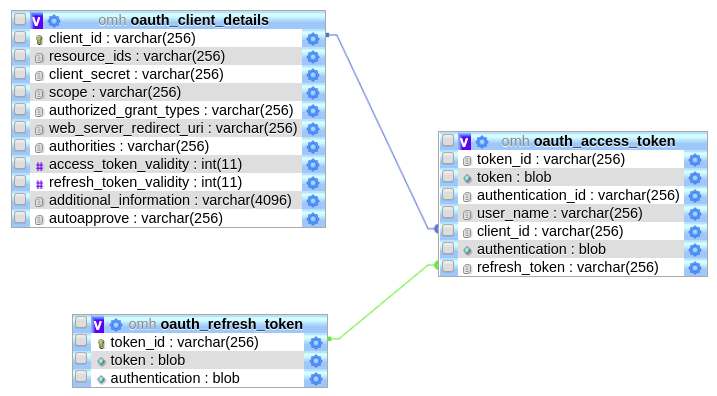
\includegraphics[width=0.8\textwidth]{imgs/auth-diagram.png}
  \caption[Diagrama do modelo de dados para guardar as credenciais dos clientes e os tokens de acesso]{Diagrama do modelo de dados para guardar as credenciais dos clientes e os tokens de acesso}
  
  \label{f:auth-diagram}
\end{figure}

\subsubsection{API REST}
Na tabela seguinte temos disponível os métodos disponíveis do servidor de autorização e autenticação.
\begin{table}[H]
\label{t:apirest-auth}
\centering
\begin{tabularx}{1\textwidth}{|p{0.3cm} p{14.4cm}|}
\multicolumn{2}{l}{\textbf{domain:port/users}}  \\ \hline 
 & Serviço POST, para criação de novos utilizadores \\
 & Recebe um JSON composto por dois campos um ''username'' e ''password'' \\ \hline
\multicolumn{2}{l}{\textbf{domain:port/oauth/token}} \\ \hline
 & Serviço POST, utilizado para efetuar o pedido de um novo token de acesso \\
 & Recebe por parâmetros o ''username'', ''password'' e o ''grant\_type'' \\ \hline
\end{tabularx}
\caption{Tabela com a API REST do servidor de autorização e autenticação}
\end{table}

\subsection{Servidor de recursos (dataPoint REST API) }
O servidor de recursos disponibiliza uma \gls{REST} \gls{API} para criação, consulta e eliminação de dataPoints. Estes dataPoints estão a ser guardados numa base de dados Mongo numa coleção com o nome dataPoint. A maior vantagem de utilizar uma base de dados não relacional é que os esquemas de dados podem ser extendidos à vontade que não é necessário efetuar nenhuma alteração ao esquema da BD. \par 
Como foi referido na fase exploratória do \gls{OMH} \ref{cap4:exp-omh} estes dataPoints são compostos por um cabeçalho e por um corpo. Este corpo é formatado pelo esquema de dados (dataschema) associado e definido no cabeçalho do dataPoint. Como foi referido também na fase exploratória foi desenvolvido um validador que verifica se o corpo do dataPoint está de acordo com o dataschema definido no cabeçalho do mesmo. \par
Estava então em falta alguns esquemas de dados para conseguirmos abranger todos os dados que precisávamos de inserir, assim como: \gls{ECG}, dados demográficos e acelerómetro. Estes dataschemas foram criados com base da informação retirada da definição da \gls{API} do \gls{FHIR} e vou mostrar de seguida como exemplo o esquema de dados criado para definir o formato de dados para as entradas para o \gls{ECG}. \newpage
\subsubsection{dataschema ECG}
\begin{figure}[H]
\inputminted[fontsize=\scriptsize]{json}{code/ecg.json}
\caption[Novo esquema de dados relativo ao ECG]{Novo esquema de dados relativo ao ECG}
\label{f:ecgjsonschema}
\end{figure}

\subsubsection{API REST}

\begin{table}[H]
\label{t:apirest-data}
\centering
\begin{tabularx}{1\textwidth}{|p{0.3cm} p{14.4cm}|}
\multicolumn{2}{l}{\textbf{domain:port/v\{apiVersion\}/dataPoints}}  \\ \hline 
 & Serviço POST, para criação de novos dataPoints \\
 & No header recebe o access\_token para o servidor de autorização para lhe dar acesso ao pedido efetuado \\
 & Recebe um documento JSON constituído por um cabeçalho e um corpo \\ \hline
\multicolumn{2}{l}{\textbf{domain:port/v\{apiVersion\}/dataPoints/id}} \\ \hline
 & Serviço DELETE, utilizado para efetuar a eliminação de um dataPoint \\
 & No header recebe o access\_token para o servidor de autorização para lhe dar acesso ao pedido efetuado \\
 & O id do dataPoint tem que ser referido no url \\ \hline
 \multicolumn{2}{l}{\textbf{domain:port/v\{apiVersion\}/dataPoints/id}} \\ \hline
 & Serviço GET, utilizado para efetuar a consulta de um dataPoint \\
 & No header recebe o access\_token para o servidor de autorização para lhe dar acesso ao pedido efetuado \\
 & O id do dataPoint tem que ser referido no url \\ \hline
 \multicolumn{2}{l}{\textbf{domain:port/v\{apiVersion\}/dataPoints/caregiver}} \\ \hline
 & Serviço GET, utilizado para efetuar a consulta dos vários dataPoints de um determinado tipo de um utilizador em específico \\
 & No header recebe o access\_token para o servidor de autorização para lhe dar acesso ao pedido efetuado \\
 & Recebe por parâmetros o ''schema\_namespace'', ''schema\_name'', ''schema\_version'', ''user\_id'' e o ''CAREGIVER\_KEY'' \\ \hline
 \multicolumn{2}{l}{\textbf{domain:port/v\{apiVersion\}/dataPoints}} \\ \hline
 & Serviço GET, utilizado para efetuar a consulta dos vários dataPoints de um determinado esquema de dados \\
 & No header recebe o access\_token para o servidor de autorização para lhe dar acesso ao pedido efetuado \\
 & Recebe por parâmetros o ''schema\_namespace'', ''schema\_name'' e o ''schema\_version'' \\ \hline
\end{tabularx}
\caption{Tabela com a API REST do servidor de recursos}
\end{table}


Todos os esquemas de dados disponíveis estão no diretório \cite{schemas-available} e estes são os tipos de dados que são utilizados para validar os dataPoints inseridos, ou seja, estes são todos aqueles que podem ser inseridos na coleção do Mongo.

\subsection{Comunicação com módulos externos}
No processo de inserção de novos dataPoints, depois de validados eles são reencaminhados para um endpoint \gls{REST}. É enviado um documento \gls{JSON} composto pelo esquema utilizado para validar o documento, como por exemplo "heart-rate" e um corpo do dataPoint inserido. Este documento é então inserido no ''EventBus'' do Vert.x, neste momento clientes podem se registar neste EventBus e verificar e analisar da maneira que quiser os dados inseridos. \par
Isto pode ser importante para por exemplo ser desenvolvido um módulo que tenha a capacidade de verificar se um utilizador que está a fazer a colheita dos dados está a sofrer de Arritmia cardíaca.
O projeto é então composto por dois verticles em que num dois verticles cria um endpoint \gls{REST} e permite publicar os mesmo Eventbus assim que os recebe.

\subsection{Como instalar este backend}
Relativamente ao servidor de autorização/autenticação e ao servidor de recursos o código está no github \cite{omh-code} e é um ''fork'' do projeto desenvolvido pela \gls{OMH}, está documentado como pode ser instalado e executado \cite{omh-runnatively}.
O código relativo à extensibilidade com módulos externos também está no github\cite{restpubsub} este projeto é composto apenas por dois verticles para os correr pode ser também por terminal e basta correr os comandos:
\begin{itemize}
    \item vertx run SimpleREST.java -cluster
    \item vertx run Receiver.java -cluster
\end{itemize}
O Receiver.java pode ser substituído ou adicionado por um outro módulo desenvolvido para receber outro tipo de esquemas de dados e os analisar.

\section{Implementação da aplicação móvel}
\subsection{Versões alvo}
Esta aplicação móvel foi desenvolvida com o intuito de conseguir abranger grande maioria dos utilizadores, suporta da versão 16 à versão 25, ou seja,  desde o Android 4.1 (Jelly Bean) até ao Android 7.1. De acordo com as informações disponíveis na plataforma de desenvolvimento do Android atinge mais de 98\% dos utilizadores \cite{android-versions}.

O projeto tem um ficheiro por defeito designado por "build.gradle", que é o local onde esta configuração é efetuada, um excerto deste ficheiro de configuração pode ser visualizado na tabela \ref{t:defaultconfig}.


\begin{table}[H]
\centering
\begin{tabular}{llll}
\hline
 & \multicolumn{2}{l}{defaultConfig \{}                                     &  \\
 &    & applicationId {\color[HTML]{009901} ''pt.ua.ieeta.healthintegration''}                       &  \\
 &    & minSdkVersion {\color[HTML]{0767D2}16}                                                    &  \\
 &    & targetSdkVersion {\color[HTML]{0767D2}25}                                                 &  \\
 &    & versionCode {\color[HTML]{0767D2}1}                                                       &  \\
 &    & versionName {\color[HTML]{009901}''1.0''}                                                   &  \\
 & \} &                                                                     & \\
\hline
\end{tabular}
\caption[Excerto da configuração padrão da aplicação móvel]{Excerto da configuração padrão da aplicação móvel}
\label{t:defaultconfig}
\end{table}


\subsection{Depêndencias}
\subsection{Tecnologias integradas e fontes de dados}
\subsection{Componentes da aplicação Android}
\subsection{Interações suportadas }


\section{Implementação da aplicação de revisão}
\subsection{Tecnologias integradas}
%linguagens, bibliotecas, frameworks,..., usados na implementação desta parte


\subsection{Componentes da aplicação HTML5??}
%mostrar a organização do projeto de código, em termos da linguagem de programação em concreto

\subsection{Interações suportadas }
%mostrar a organização do projeto de código, em termos da linguagem de programação em concreto






\section{Como aplicar e estender a plataforma em novos contextos}

% explicar como se pega no que ficou feito para usar num novo projeto e como se pode estender (e.g: para novos tipos de dados)

\subsection{Criar um novo tipo de dados}

A criação de um novo tipo de dados pode ser feita com a ajuda do repositório ''schemas'' \cite{schemas-rep} que foi criado pela organização da \gls{OMH}. Para isto vai necessitar de algumas ferramentas entre elas: o git \cite{git-install} para puxar o repositório; o Java 8 \cite{java-overview} para executar o validador; um editor de texto como por exemplo o atom \cite{atom-install}. Vou descrever agora a lista de tarefas para conseguir efetuar a criação de um novo tipo de dados. Para este tutorial vou criar o tipo de dados acelerómetro. É um dos tipos de dados que são obtidos através do VitalJacket.

\begin{enumerate}
  \item Clonar o repositório correspondente para um diretório à sua escolha com o comando \par
  ''git clone https://github.com/openmhealth/schemas'' 
  De seguida vamos fazer duas coisas principais: uma delas é criar o ficheiro que define o novo tipo de dados; a outra é criar um ficheiro com uma amostra do novo tipo de dados.
  \item Criar um ficheiro que define o tipo de dados em \gls{JSON} schema, para isso, adicione um novo ficheiro no diretório schema/omh. O nome deste ficheiro tem que ser composto pelo nome que quer dar ao tipo de dados e a versão correspondente, tem que terminar com a extensão .json. No meu caso criei com o nome accelerometer-1.0.json  \par A versão escolhida aqui é a 1.0 mas podia ser qualquer outra. Pode reparar que no diretório schema/omh tem acesso a todos os ficheiros que definem todos os tipos de dados.
  \item Adicionar uma nova pasta ao diretório testdata/omh como o nome respetivo ao ficheiro criado anteriormente. Neste caso criar uma pasta com o nome accelerometer.
  \item Vai agora criar uma pasta correspondente à versão introduzida no ponto 2. Neste caso é 1.0 e uma outra pasta dentro da criada anteriormente com o nome shouldPass.
  \item Dentro do diretório shouldPass vai ter que criar um ou vários ficheiros para ser utilizados como amostras do tipo de dados. O objetivo deste diretório é ter várias amostras válidas testando-as com o tipo de dados criado no ponto 2. Para este tutorial criei o ficheiro example.json. \par Neste ponto o nome do ficheiro é opcional só tem que acabar com a extensão .json
  Como criou o diretório shouldPass, pode também criar o diretório shouldFail criando também vários ficheiros para testar o tipo de dados criado. \par 
  Neste ponto tem tudo preparado para começar a criar o novo tipo de dados e validar a amostra com a nova definição do novo tipo de dados criados.
  
  \begin{figure}[!ht]
  \centering
  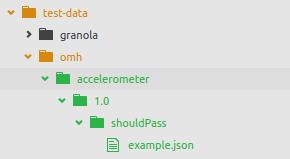
\includegraphics[width=0.5\textwidth]{imgs/newsampledata.png}
  \caption[Esquema de diretório para o novo sample]{Esquema de diretório para o exemplo do novo tipo de dados}
  
  \label{f:directorynewsample}
\end{figure}
  
\item Vamos agora preencher o ficheiro com a definição do novo tipo de dados, aquele que criou no ponto 2. O ficheiro vai ser criado no formato de \gls{JSON} schema. Para suportar a criação deste ficheiro pode reutilizar schemas existentes \cite{schema-library} e referênciá-los, deste modo estará a criar um modelo com tipos de dados normalizados. No meu caso vou reutilizar um schema para definir a data/hora e um outro para definir o tipo de atividade que está a efetuar no momento da leitura. Os restantes dados estão relacionados com o acelerómetro em si, a sessão e a leitura respetiva.
O ficheiro fica do seguinte modo: 

\begin{figure}[H]
\inputminted[fontsize=\scriptsize]{json}{code/accelerometer-1.0.json}
\caption[\gls{JSON} schema para o novo tipo de dados de acelerómetro]{\gls{JSON} schema para o novo tipo de dados de acelerómetro}
\label{f:accelerometer-json-schema}
\end{figure}

\item Preencha o ficheiro com uma amostra do novo tipo de dados, para isso tem que ter em conta a definição utilizada, pois porque se esta amostra não for compatível não vai passar no validador.

\begin{figure}[H]
\inputminted[fontsize=\scriptsize]{json}{code/example.json}
\caption[Exemplo do tipo de dados de acelerómetro]{Exemplo do tipo de dados de acelerómetro}
\label{f:accelerometer-json-data}
\end{figure}

\item Para compilar e executar o validador tem que executar o comando ''./gradlew test-data-validator:bootRun'' no diretório principal ''schemas'' ou então execute o comando ''./gradlew bootRun'' no diretório ''schemas/test-data-validator''. 

\subsection{Como utilizar o novo tipo de dados criado}

Para adicionar o novo tipo de dados criado, tem que o integrar com os restantes tipos de dados existentes. \par Tendo em conta que já tem o repositório omh-dsu-ri clonado através do comando ''git clone https://github.com/luistduarte/omh-dsu-ri', terá que copiar o seu novo tipo de dados para o diretório ''omh-dsu-ri/resource-server/src/main/resources/schema/omh'' que é onde se encontram os restantes tipos de dados válidos.

\end{enumerate}

\cleardoublepage
